\cleardoublepage
\singlespacing
\chapter{BACKGROUND}
\label{c:background}
\doublespacing\nointerlineskip

\section{Internet-of-Things}

\subsection{What is Internet-of-Things}

Internet-of-Things is a powerful paradigm in the scenario of modern wireless
telecommunications. It refers to the pervasive presence of uniquely identifiable
objects (things) around us - such as Radio Frequency IDentification (RFID)
tags~\cite{Shepard2005}, sensors, actuators, mobile phones, which would be able
to interact with each other forming a network like
structure~\cite{Atzori20102787}. Example scenarios where IoT would shine: alarms
clock goes off early if there is traffic; plants communicate to the sprinkler
system when it's time for them to be watered; running shoes communicate time,
speed and distance so that their wearers can compete in real time with people on
the other side of the world; medicine containers tell your family members if you
forget to take the medicine. The paradigm gradually leads to all objects
surrounding us to become connected to the Internet, to interact with other
connected objects on the other end of the web and have access to comparative
information which would not be possible before.

\subsection{The Evolution of Internet-of-Things}

The figure~\ref{fig:evolution} illustrates an evolution of Internet.
Communication between computers already exists that made possible for two PCs to
send messages across large geographical areas. With the Internet, all the
computers connected to the Internet can talk to each other and now with mobile
phones, the connections have become mobile.
It would be unimaginable 20 years ago, when you have to communicate with someone
far away in immediate urgency, you can open up your phone and make a call to
someone far away from you and initiate a conversation. Nowadays even more so
with 3G networks, even phones can connect to the Internet and be part of the
network.
Social media, such as email, blog, facebook, twitter, has been uniting
people on the Internet up until now. With social media, we could go beyond
physical limits with whom we can keep in direct contact. Internet-of-Things will
further make possible for massive amount of objects to be online and to enable
objects to access external information about themselves through external
services in their vicinity.~\cite{Associati2011a}

\begin{figure}[h!]
\centering
    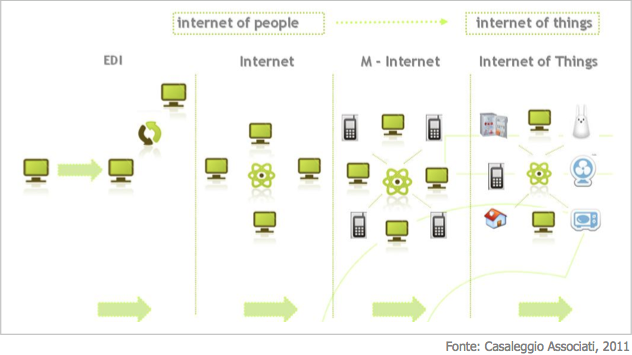
\includegraphics[width=\linewidth]{figures/evolution}
\caption{The Evolution from Internet of People to Internet of Things}
\label{fig:evolution}
\end{figure}


\subsection{Potential Applications}

Today more things than humans are connected to the Internet~\cite{CISCO}. It is
estimated things will have 24 billion devices connected to the Internet by
2020~\cite{Malik}. In addition, the computation capabilities per device are
increasing. Today's smart phones are about 15 times faster than CPUs used in
1979 Cray-1~\cite{Randomly2010}. 

Potential applications of this new emerging paradigm is skyrocketing as more
sensor networks, actuators, have been more common as sensing, communication, and
analytics have matured that are ubiquitously embedded into everyday objects
surrounding every where we go. Some examples are highlighted below:
\begin{enumerate}
\item Smart Home: At home, embedded sensors can sense human presence and could
understand human activities to properly adjust air quality and temperature by
commanding the air conditioner on or off to save energy without sacrificing
human comfort.
\item Economical agriculture: In a vast farm land, remote sensors can detect and
identify the outbreak of pests and initiate spreading pesticide at only the
areas of outbreak.
\item Vehicle safety: Sensors on the car can help drivers understand its own
driving conditions and monitor driver condition to help others to understand
driver's condition to prevent traffic accidents.
\end{enumerate}

In conclusion, connected embedded things could enhance people's lives
tremendously in a way never seen before. This paradigm shift creates numerous
opportunities and challenges for engineering~\cite{Chen2012}.

\subsection{Challenges}

In the future, enormous amount of sensors, actuators, or things will be
deployed. The cost of serving such amount of things will be a major concern. One
big challenge is to reduce and minimize costs to deploy and maintain the system.
Many domestic ubiquitous computing projects have failed because of high
complexity in sensor network deployment~\cite{Beckmann2004}.

Once the network of sensors have been deployed, it is almost always impossible to
perform manual effort to repair such as battery replacement, case
replacement. Therefore, another challenge is low power sensor design, or
self-sustainable design eliminating the needs for battery over the lifetime of
sensors. For example, if the sensors are deployed in mountain range where human
contact is costly, the lifetime of sensors should last as long as the lifetime
of the project.

After the data has been collected, the sensors will communicate the data
collected with other parts of the network. Since the number of sensors have far
exceed the number of humans, and this gap will only accelerate faster in the
future~\cite{CISCO}, it is a challenge to serve the huge amount of data
generated by sensors when the base station can only provide quality of service
up to an arbitrary threshold. The ability to provide critical analytics to the
ocean of data generated by IoT will be a key role in the new computing era.

\section{Wireless Sensor Networks}

\subsection{What is Wireless Sensor Networks}

Wireless sensor network (WSN), a M2M network, consists of a network of sensor
nodes, where each is uniquely identifiable. Each sensor node is equipped with
low-power, low-cost, and failure-prone sensors or actuators.  Sensor nodes
collaborate to collect, process and disseminate environmental
information\cite{ArchanaBharathidasan}.

Sensor network could be homogeneous, meaning all nodes are identical with same
sensors, actuators and hardware setup. Sensor networks could also be
heterogeneous where nodes have different sensors, actuators and hardware setup.
Heterogeneous networks require higher level management and organization
resources. Wireless sensor nodes could communicate wirelessly through air by
sending electronic signals. Wireless communications aren't stable, as it is
highly influenced by environmental factors.

\subsection{Benefits of Decentralized Architecture}

In general, centralized architecture is easy to implement but if the central
node failed, the whole system would went down. A decentralized architecture
might be more expensive to design, implement and more delicate to manage, but it
is easier to scale and become more robust. In a decentralized architecture, each
node capture a localized measurement. As the number of sensor node increases,
     the system could provide much greater accuracy and finer resolution in the
     information gathered compared to what a single sensor would obtain over
     a period of time.

In addition, new sensor nodes could be added to the network dynamically, and
the system could continue to provide services. If a sensor node failed, nearby
nodes could substitute for it and keep capturing the local information.
Redundancy, or failover mechanism, is desirable as it makes the system more
fault tolerant.

\subsection{Challenges}

Most of the challenges in WSN are similar to the challenges in building IoT
system.  However, in addition to the challenges above, it is difficult to
develop a complex distributed applications with low end hardware and low end
programming language. Most programming environments have been designed to work
for a monolithic system that executes one instruction at a time in contrast to
distributed systems with multiple instances of the program running
asynchronously and each is prone to failure.

\subsubsection{Service-Oriented Architecture for Wireless Sensor Network}

Service-oriented architecture (SOA) is an established approach which eases the
development of complex distributed applications. Using the concept, sensor
network applications are composed of successively of independent software
building blocks (services) which are situated on the sensor nodes in order to
perform predetermined tasks.~\cite{Neumann2010, Marin-Perianu2007} SOA provides
an easy-to-use interaction paradigm and decouple the application from the
low-level technologies.

\section{WuKong: The intelligent middleware for M2M applications}

\subsection{Goal}

Deployment and development for M2M applications are in its infancy today, as
many applications are still single purpose in homogeneous networks with
specific network protocols. The hardware has a fixed range of sensors, and the
applications cannot be easily ported to other platforms.

The existing middleware support that decouple high-level application design
abstractions and low-level hardware has not been successful.

In Intel-NTU Center Special Interest Group for Context Analysis and Management 
(SIGCAM), we have been collaborating on a project, called WuKong, aiming to develop 
an intelligent middleware for developing, and deploying machine-to-machine 
(M2M) applications with ease. The main goal of this project is to support
intelligent mapping from a high-level logical component flow (FBP) to
self-discovered devices with selected network connections a target
environment\cite{Reijers}.

\subsection{Flow Base Programming}

M2M applications are by definition distributed where the application
requirements involve a network of nodes collaborating for some common 
goals. M2M applications are typically defined by its flow of information
between components, as opposed to more traditional applications that focus more
on local information processing.

Flow Base Programming (FBP) is best suited for describing M2M applications as it
allows the developers for the applications to focus more on the
abstraction meaning of the components instead letting the unimportant details
such as the hardware to stick right in the face. The result application will
contain all necessary information for the framework to construct low-level
details to implement the flow.

Applications are designed and constructed on FBP canvas by dragging a set of
abstract components from the library as illustrated in
figure~\ref{fig:fbp-application}. Each component is illustrated by a green
block, each block has a set of properties, each with different access modes,
such as \textit{readonly}, \textit{writeonly}, \textit{readwrite}. Properties on
the left of the green blocks are properties that could be written, and
properties on the right are readable. Components are connected by links, which
is drawn by linking two properties in different components.

Some components represent physical hardware such as sensors, or actuators
while some other components represent virtual processes such as
mathematical computations, comparisons, etc. However, the final physical implementations
of the components are only made during application deployment by the Master but
not during FBP construction.

Components expose their interface through properties. A link can only made with
properties with matching data type. The FBP application in
figure~\ref{fig:fbp-application} illustrates a simple scenario where the light
actuator will turn on the light if light level drops below some value. The
Numeric Controller component will be assigned to a user input device used by
users to set its desire light threshold, which its output is sent to Threshold
component. The light value is sensed from Light Sensor component and sent to
Threshold. If the light value sensed is below the threshold value, Threshold
will output a boolean to set the on off property of Light Actuator to turn the
device, which will be determined during deployment, that it is represented by on
or off.

\begin{figure}[h!]
\centering
    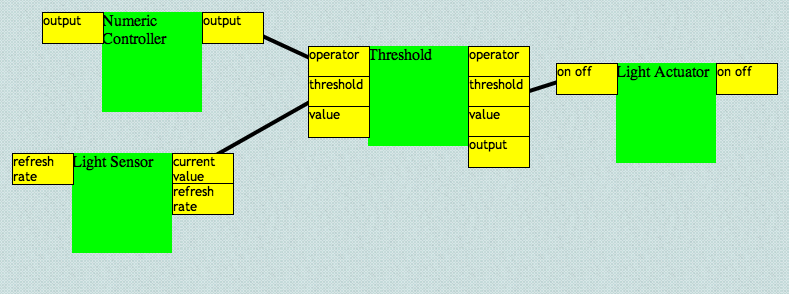
\includegraphics[width=\linewidth]{figures/fbp-application}
\caption{A FBP application}
\label{fig:fbp-application}
\end{figure}

\subsection{Sensor Profile Framework}

While FBP defines the logical view of an application, Sensor Profile
Framework allows tracking, identification of physical resources within the
sensor network.  There are a range of sensors which provide similar
functionality with different level of quality. Sensor Profile Framework
could model the sensor capability to enable handling heterogeneous sensors and
provide a common abstraction for the logical view.

There are two main concepts in Sensor Profile Framework, WuClasses and
WuObjects. WuClasss model components by exposing a number of properties
describing, and allow access to, a specific resource represented by the class.
For example, from drawing from the example in Figure~\ref{fig:fbp-application},
the on off property of Light Actuator component is boolean writeonly. WuClass
also implements an update function to describe a component's behavior. For
example, Threshold has four properties: operator, threshold, value, output. The
output value is determined from the previous 3 properties that it returns true
when the value is lower or higher than the threshold which depends on the value
of the operator, and it returns false otherwise.


WuObjects are the main unit of processing that are hosted on the nodes. Each
WuObject is an instance of a WuClass. Both concepts allow the framework to
achieve 4 responsibilities:
\begin{enumerate}
\item Allow the Master to discover the current status of a node with the list
of WuClasses and WuObjects it has.
\item Create new WuObject instances on a node to start receiving data and doing
local data processing.
\item Trigger executions in WuObjects, either periodically or as a result of
changing inputs.
\item Propagate changes of properties between linked properties in different
components, which may be hosted locally or remotely.
\end{enumerate}

\subsubsection{Property Propagation}

Sensor Profile Framework is in charge of communication between WuObjects as
well, which are not necessarily on the same nodes. It monitors
the changes in properties and propagates the changes to the connected WuObjects.
For example, if a Temperature WuObject is connected to a Threshold WuObject,
the changes in Temperature current value property will trigger propagation from
the framework to propagate the new value in current value to the
Threshold WuObject connected property, and since Threshold WuObject could be on
a different node, the framework will take care of this by initiating
a wireless connection between the nodes to send the data over. Once a new value
has been set, Threshold WuObject will also trigger its update() function to
recompute its output properties which in turn would cause another chain of
propagation to the linked WuObjects.

\subsection{Compilation and Mapping}

Figure~\ref{fig:wukong-flow} shows the overview of WuKong build flow. The
left part represents the build process for NanoKong VM which will be installed
on the sensor nodes as part of the WuKong framework. The top part represents
the build process for generating component libraries and Virtual WuClass
library which will be used in other parts of the process. The right part
illustrates the build process for FBP applications from being drawn in the IDE
to Java bytecode that will be transmitted to the nodes.

The FBP program from the IDE will be exported as XML to the Master, the Master
will then take this XML and passed to Mapper to generate a Java program that
will be executed on the nodes. Finally, the compiled code is then wirelessly
uploaded to the nodes in the network.

The Java code consists of many parts from different phases of the mapping process.
First, the Java code contains information about links between components that
were taken from the FBP XML passed in earlier from the IDE. A link contains the
source component id, destination component id. The library code for components
corresponding to the component ids are stored in the node if it is written in
native language, or uploaded as part of the Java bytecode if it is written in
Java language. Second, it contains information about the mapping from
application component ids to actual node identifications and positions. The
purpose of a mapping which separates from the actual link makes it easier to
substitute the actual host of the WuObject later during
reconfiguration from the Master. This mapping is created by the Master during
discovery phase that probe the network for node's capabilities in terms of
available WuClasses, then mapper will decide the final candidates that will be
hosting for a component. If no native version of a component is found on the
nodes, mapper will substitute with a Java version of it.

\begin{figure}[h!]
\centering
    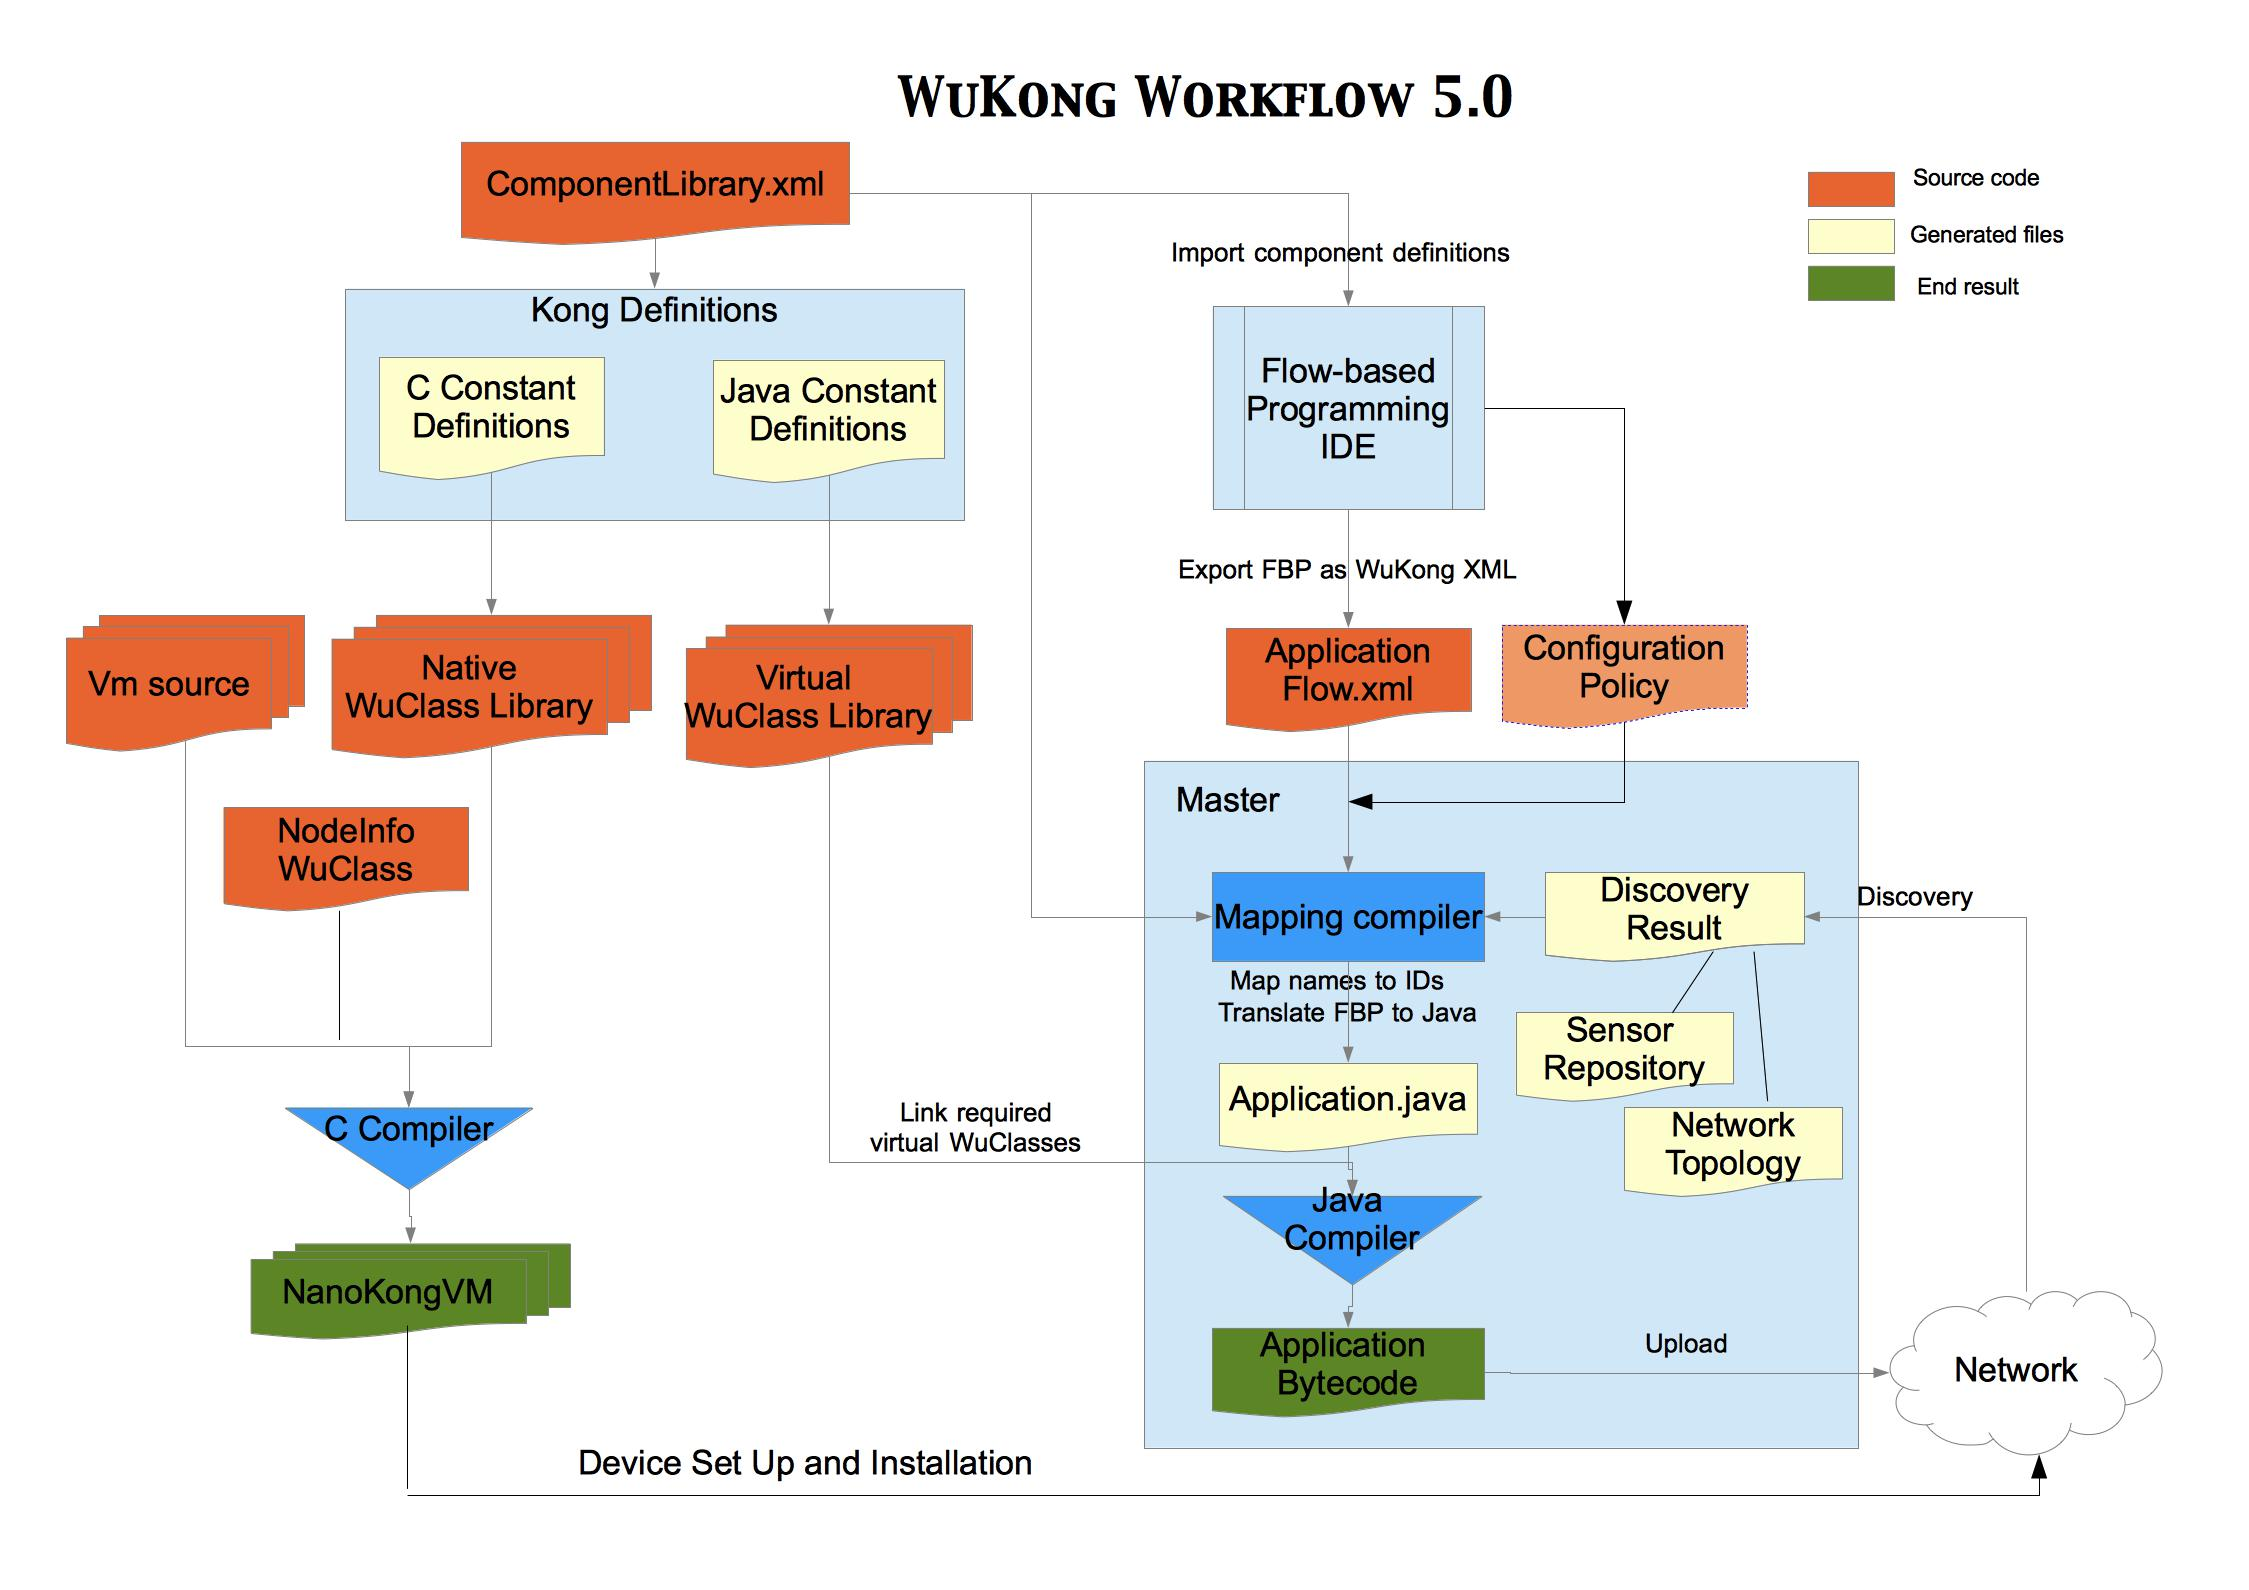
\includegraphics[width=\linewidth]{figures/wukong-flow}
\caption{WuKong application build flow}
\label{fig:wukong-flow}
\end{figure}

\subsection{System Progression Framework}

There are a few popular wireless communication protocols in M2M applications:
ZigBee, ZWave. It is expected that in the future more diverse
wireless nodes equipped with radios that support protocols such as low-power
Bluetooth and WiFi that all have one or more powerful gateway to connect to the
outside world. In WuKong system, one of the gateways will take on the role of
higher management decision maker called \emph{Master} to making the decisions for
deployment and producing the configuration of WSNs.


\begin{comment}
\section{Redundancy Architecture}

%A distributed system usually consists of hosts that host services that clients or
%other services could read or write with some associated communication
%frequencies according to the application requirements. The
%problem of partial failures makes service redundancy a fundamental technique to
%distributed systems as it improves availability, eliminates single points of
%failure. A system that is hardwired to get data from node X will fail when
%X fails. The problem of designing a system with replicas where node Y, which
%can provide the same service as X, can take over when X fails. To design such
%system, it is important to have a clear definition of a service such that it
%could be replicated onto heterogeneous hosts. It is
%also essential that the system could track and manage available replicas in the
%network. Autonomy is an important attribute of distributed systems since most
%of them would be left unattended for a long period of time; systems should be
%able to reconfigure and recover themselves in the event of failure.

Sensor networks are usually deployed in large scale and unattended in long
period of time. Sensor networks communicate with
low-power wireless radios to aid scientists in collecting spatial data that
could lead to more understanding of the environment. However, several
challenges such as node failures, message loss, and sensor calibration leaves
the effectiveness of sensor networks in question. With the assumption of spare
homogeneous resources, redundancy is used in sensor networks to increase fault
tolerance against node failures. The system is designed with backup nodes that
could automatically recover and replace should one node fail.
\end{comment}
